\section{Problem Setups}
Due to the inherent limitations of current computing systems, 
obtaining sufficiently precise solutions is both computationally expensive and time-consuming. 
These challenges arise from the constraints imposed by the clock speed of computing units, 
as described by 
Moore's Law \cite{Moore_Law}, 
as well as the relatively low communication speeds between these units. 
While modern numerical methods have advanced to a level where they can produce 
satisfactory results within acceptable time frames across many research domains, 
the increasing scale of problems we aim to solve has driven the search for more 
cost-effective approaches. This has led to a growing interest in neural networks as a promising alternative.

In this project, I aim to evaluate the performance of the Finite-Difference Time-Domain (FDTD) 
method and the Physics-Informed Neural Network (PINN) model within parallelized computing 
environments by find the steady-state solution of PDEs.
These two methodologies broadly represent the current approaches to 
handling PDEs, specifically 
CPU-based parallelization and GPU-based parallelization.

\subsection{General Form}\label{SEC_General_Form}
Starting with the general form of the PDEs, rather than the specific euqations, is because 
different equations give perform differently on the same compute system.
To this end, consider the previously discussed form of PDEs shown in 
equation \ref{EQ_General_PDEs} which parametrized by number $\lambda$ and an operator $\mathcal{N}[\cdot; \lambda]$.
Moreover, we assume the variable $x$ is a 2D or 3D spatio vector which is written in 
$\vec{x} \in \mathbb{R}^d$, $d = 2, 3$.
\begin{align}\label{EQ_General_Form_PDE}
  &\frac{\partial u}{\partial t}\left(t,\vec{x}\right) + \mathcal{N}\left[u(t,\vec{x});\lambda\right] = 0, &\vec{x}\in\Omega, &t\in[0, +\infty) \nonumber\\
  &u\left(0,\vec{x}\right) = \varphi (\vec{x}), &\vec{x}\in\Omega & \\
  &u\left(t,\vec{x}\right) = g (t,\vec{x}),     &\vec{x}\in \overline{\Omega}, &t\in[0, +\infty) \nonumber
\end{align}
The domain of this PDE system is considered between $0$ and $1$, where is denoted with $\Omega = [0, 1]^d$, $d = 2,3$.
To these setups, we have the general form of the PDEs we are going to investigated, shown in equations \ref{EQ_General_Form_PDE}
The boundary condition shown in E.q. \ref{EQ_General_Form_PDE} is Dirichlet Condition known as first type boundary condition, where as the 
second type boundary condition (Von Neumman) [E.q. \ref{EQ_Von_Neumman_BC}] gives the other form of $u(t,\vec{x})$ at the boundary $\overline{\Omega}$.
\begin{equation}\label{EQ_Von_Neumman_BC}
  \frac{\partial u}{\partial \vec{x}} = g(t, \vec{x}),\:\: \vec{x}\in \overline{\Omega}, \:\:t\in[0, +\infty)
\end{equation}

\subsection{Specific Form}\label{SEC:Specific_Form}
With general form proposed in section \ref{SEC_General_Form}[E.q. \ref{EQ_General_Form_PDE}],
I specify a particular form of this heat problem to help us to have better understand the quality of our 
solutions and programs.
In $2$ dimension space, the domain $\Omega = \left[ 0, 1\right] ^2 \in \mathbb{R}^2$ and its boundary
denoted with $\overline{\Omega}$, the initial condition $\varphi(x,y) = 0$.
such problem has the certain form below
\begin{align}\label{EQ:Heat2D}
  &\frac{\partial u}{\partial t} = \alpha \left(
    \frac{\partial u^2}{\partial^2 x}
    +
    \frac{\partial u^2}{\partial^2 y}
  \right) &(x,y) \in \Omega, \: t \in \left[0, +\infty\right)  \nonumber\\
  &u(0,x,y)  = \varphi(x,y) = 0 &(x,y) \in \Omega\\
  &u(t,x,y)
   = g(x,y)
   = \begin{cases}
    y, \:\: x=0, y\in\left(0,1\right)\\
    1, \:\: x=1, y\in\left(0,1\right)\\
    x, \:\: y=0, x\in\left(0,1\right)\\
    1, \:\: y =1, x\in\left(0,1\right)
  \end{cases}
  &t \in \left[0, +\infty\right) \nonumber
\end{align}
With given format, and $\alpha = 1$, we have the analytical solution of this equations, where is 
\begin{equation}\label{EQ_SOLUTION_2D}
  u(t,x,y) = x + y - xy, \:\:(x,y) \in \Omega,\: t \in \left[0, +\infty\right)
\end{equation}
In 3 dimension space, similarly, with identical initial condition set up to $0$, coefficient $\alpha = 1$,
the boundaries are 
\begin{equation} \label{EQ:Heat3D}
  u(t,x,y,z) = g(x,y,z) = 
  \begin{cases}
    y+z -2yz        , \:\: &x=0,\\
    1 - y - z + 2yz , \:\: &x=1,\\
    x+z - 2xz       , \:\: &y=0,\\
    1 - x - z + 2xz , \:\: &y =1,\\
    x+y - 2xy       , \:\: &z=0,\\
    1 - x - y + 2xy , \:\: &z=1
  \end{cases}
  \:\:, t \in \left[0, +\infty\right)
\end{equation}
In such case, the analytical solution has for form below 
\begin{equation}
  u(t,x,y,z) = x + y + z - 2xy - 2xz - 2yz + 4xyz, \:\:(x,y,z) \in \Omega,\: t \in \left[0, +\infty\right)
\end{equation}


\subsection{Discretization}
To begin with discretizing the objects or regions we intend to 
evaluate via matrices, we consider a straightforward approach: 
using the coordinates in $d=2,3$ dimensional spaces and the function 
values at those points to simplify the objects. 
This naive approach works well for investigating objects with regular shapes, such as a cube.

For the FDTD (Finite-Difference Time-Domain) method, we use a finely 
generated $d$-cube with shape $\left\{n_i\right\}_i^{d}$. Including 
the boundary conditions, the cube has $\prod_i (n_i+2)$ nodes. 
It requires $4\prod_i (n_i+2)$ bytes for float32 or $8\prod_i (n_i+2)$ bytes 
for float64 to store in memory. 
With this setup, for equally spaced nodes, we have:
\begin{equation}
  \Delta x_i = \frac{1}{n_i-1}
\end{equation}

Unlike the previously generated regular grid of 
points with dimensions $n_xn_yn_z$, 
another strategy is to randomly generate the same number of points based on the same known conditions, 
covering both the central part and the boundary. 
In this scenario, 
shown in figure, 
there are $n_x n_yn_z$ central points, 
with function values set according to the boundary conditions, 
and $2 \times(n_xn_y + n_yn_z + n_zn_x)$ boundary points to be solved. 
This set of points can be used for training a PINN model.

% 不同于之前生成规则的nx * ny * nz的点阵,另一种策略是对于与先前同样的已知条件随机生成同样数量的点,用于中心的部分以及边界部分。
% 这种情况下一共有nx * ny * nz个中心部分,根据边界条件设置函数值,以及(nx * ny + ny * nz + nz * nx)*2个边界点,需要求解的部分。
% 这种方式生成的点集用于训练PINN模型。
% \begin{figure}[htbp]
%   \centering
%   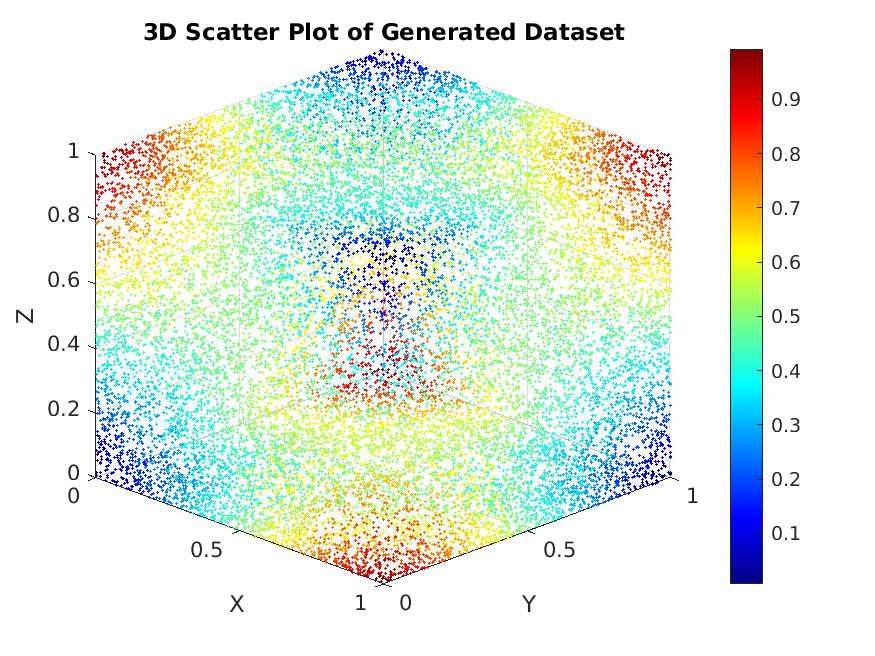
\includegraphics[width=0.5\textwidth]{figure/FIG_main2_dataset.png}
%   \caption{Randomly general dataset for 3D PINN model training.}
%   \label{FIG_Topology_Callan}
% \end{figure}

% \begin{figure}[htbp]
%   \centering
  
%   \caption{Figure Shows the FDM idea, If NEED}
%   \label{<label>}
% \end{figure}


% \subsection{Accuracy}
% When we tried to represent numbers using arithmetic in binary, decimal or hexadecimal, truncation always affects the precision of every number, 
% or so called as 
% round-off-error.

% \subsubsection{Round-off Error}
% In IEEE-754 \cite{IEEE_754} standards, a $32$-bit floating pointer number, single precision, obligatorily represented with $23$-bit mantissa, 
% $8$-bit exponent and $1$-bit for sign. 
% Where as $64$-bit floating number, double precision, also ubiquitous used, which has $11$-bit exponent and $52$-bit mantissa.
% After almost three decades development, not only single and double precisions (float32, float64) are ubiquitously in use, 
% also more formats such as fp4, fp8, and fp16 etc. Both of them follows the simple form of exponent $k$, sign $n$ and mantissa $N$. 
% \cite{IEEE_754_p2_eq1}
% \begin{equation*}
%   2^{k+1-N}n
% \end{equation*}
% Round-off errors are a manifestation of the fact that on a digital computer, which is unavoidable in numerical computations.
% In such case, the precision of the number depends on how many bytes are used to store single number. 
% For instance, a float32 number provides $2^{-23} \approx 1.2\times10^{-7}$, and a double precision number gives $2^{-53} \approx 2.2\times10^{-16}$, 
% such number is called machine $\epsilon$ which is the smallest number the machine can represent with given format.

% In numerical methods I investigated, the FDTDs are conventionally using double precision number so that the programs can treat extreamly large and small 
% numbers simultaneously in the same computation, without worring about the round-off errors.
% However, as mentioned, fp32 and fp16 are also popular use in scientific computing, especially in machine learning training process. 
% While the lasted training GPUs are integrated compute accelarate unit for low precision floating numbers. \cite{NVIDIA_HB200_PAPER}.

% \subsubsection{Floating-point Arithmetic}
% The other type loss comes from the arithmetic operations on two numbers $x$, $y$. 
% The standard model holds that 
% \begin{equation}
%   fl(x \:\text{op}\: y) = (x \: \text{op} \: y) (1+\delta), \:\:\: \left|\delta\right| < \epsilon
% \end{equation}
% where the op stands for the four elementary operations: $+, -, \times, /$. \cite{Germund,NMSC,V1,P112}.

